\documentclass[12pt,letterpaper]{article}

\usepackage[utf8]{inputenc}
\usepackage{color}
\usepackage{cite}
\usepackage{cancel}
\usepackage[normalem]{ulem}
\usepackage{stackengine}
%\usepackage{epstopdf}
%\usepackage{mathbbol}
%\usepackage{hyperref}

%%%%%%%%%%%%%%%%%%%%%%%%%%%%%%
%%% PAVLOS TEMPLATE
%%%%%%%%%%%%%%%%%%%%%%%%%%%%%%
\usepackage{amsmath,amssymb,amsthm,bm}
\usepackage[usenames,dvipsnames]{xcolor}
\usepackage{graphicx}
\usepackage[T1]{fontenc}
\usepackage{pxfonts}
\usepackage{enumerate,verbatim,cite}
\usepackage[margin=1in]{geometry}
\usepackage{fancyhdr}


\pagestyle{fancy}
\addtolength{\footskip}{\baselineskip}
\renewcommand{\headrulewidth}{0pt}
\renewcommand{\footrulewidth}{0.4pt}
\fancyhf{}
\fancyfoot[L]{\textit{Last Modified: \today}}
\fancyfoot[C]{\thepage}
\usepackage[pdftex,bookmarks,hyperfigures,colorlinks
						,urlcolor=blue
						,citecolor=blue
						,linkcolor=blue
						,pdfstartview=FitH]{hyperref}


\renewcommand{\r}{{\bf r}}
\newcommand{\dery}{\frac{dx}{dt}}
\renewcommand{\k}{{\bf k}}
\newcommand{\be}{\begin{equation}}
\newcommand{\ee}{\end{equation}}

\newcommand{\myTitleBox}{
\noindent\makebox[\linewidth][c]{%
  %
    \parbox{\paperwidth}{%
      \hspace*{\dimexpr\hoffset+\oddsidemargin+1in\relax}%
      \begin{minipage}{\dimexpr\textwidth-2\fboxsep-2\fboxrule\relax}
      {\large\textbf{\courseTitleS}\courseTitle\hfill}\vspace{2mm}\\
%      {\large\textbf{\topicsCoveredS}\topicsCovered\hfill}\vspace{2mm}\\
      {\large\courseInstructors\hfill}\vspace{2mm}\\
%      \secAuthor\hfill\sectionTimesV\\
%      \authorContact\hfill\sectionTime\\
      \end{minipage}
    %
  }%
}
}


\date{}
%%%%%%%%%%%%%%%%%%%%%%%%%%%%%
%%%%%% END PAVLOS CODE
%%%%%%%%%%%%%%%%%%%%%%%%%%%%%


% bold vectors
\newcommand{\Rset}{\mathbb{R}}

\newcommand{\xx}{{\bf x}}
\newcommand{\yy}{{\bf y}}
\newcommand{\X}{\mathbf{X}}
\newcommand{\bmu}{{\bm{\mu}}}
\newcommand{\bbeta}{{\bm{\beta}}}
\newcommand{\etab}{{\bm{\eta}}}
\newcommand{\btheta}{{\bm{\theta}}}
% 
\newcommand{\yi}{{y_i}}
\newcommand{\xxi}{x_i}
\newcommand{\mui}{{\mu_i}}
\newcommand{\thi}{{\theta_i}}
\newcommand{\phii}{{\phi_i}}
\newcommand{\ft}{{f_{\thi}}}
\newcommand{\sumi}{{\sum_{i=1}^n}}


% \newcommand{\D}{\mathcal{D}_\text{KL}}
\providecommand{\D}[2]{\mathcal{D}_\text{KL}\left( #1 ~||~ #2 \right)}

\newcommand{\yth}{(\yy|\btheta)}
\newcommand{\thM}{\btheta_\text{MLE}}
\newcommand{\thMj}{ {\btheta_\text{MLE}^{(j)}}}
\newcommand{\I}{\mathcal{I} }

\providecommand{\tr}[1]{\text{Tr}\left[ #1 \right]}



%\providecommand{\E}[1]{\text{E}\left[ #1 \right]}
\providecommand{\E}[1]{\mathbb{E}\left[ #1 \right]}
\providecommand{\Ep}[2]{\mathbb{E}_#1\left[ #2 \right]}

\providecommand{\var}[1]{\text{var}\left[ #1 \right]}

\providecommand{\tred}[1]{{\bf\textcolor{red}{#1}}}%
\providecommand{\tblue}[1]{{\textcolor{blue}{#1}}}
\providecommand{\PP}[0]{{\bf{\textcolor{red}{PP:~}}}}
\providecommand{\pp}[1]{{\bf{\textcolor{red}{[PP:~#1]}}}}
\providecommand{\mm}[1]{{\bf{\textcolor{blue}{[MM:~#1]}}}}


\DeclareRobustCommand{\bbone}{\text{\usefont{U}{bbold}{m}{n}1}}


\begin{document}
%\myTitleBox

\noindent {\small{\sc{CS 109A: Advanced Topics in Data Science}  }\\
\small{\sc{Protopapas, Rader, Tanner}} \hfill \\ }

\begin{center}
%\section*{ Likelihood Maximization \& Information Criteria: \\  Akaike Information Criterion}
\section*{Methods of Dimensionality Reduction:\\Principal Component Analysis}
\noindent {\small{\\ \small{\sc{Authors: C. Flamant, M. Mattheakis, P. Protopapas}} }}
\noindent {\small{\\ \small{\sc{Based on W. Ryan Lee's notes of CS109, Fall 2017}}}} 
\end{center}



\section{Introduction}
\label{sec:intro}

Regularization is a method that allows as to analyze and perform regression on high-dimensional data, however, it seems somewhat \emph{naive} in the following sense. Suppose that the number predictors $p$ is large, whether or not is relative to the number observations $n$. Then, the LASSO estimator, for example, would select some $p' < p$ predictors for some choice of $\lambda$. However, it is not at all clear that the chosen $p'$  predictors are the "appropriate" variables to consider in the problem. This may be clearer in light of an example taken from  \cite{shlens2003}.

{\bf Example:} Consider the spring-mass system depicted in Fig. \ref{fig.exampleSpring}, where, for simplicity, we assume that the mass is attached to a massless, frictionless  spring. The mass is released a small distance away from equilibrium along the $x$-axis. Because we assume an ideal spring that is stretched along $x$-axis, it is oscillating indefinitely along this direction. 
By understanding the physics of the problem, it is clear that there is only one degree of freedom in the system, which is indicated by the $x$-axis.  We suppose that we do not know the physics and the equations of motion behind of this experiment and, on the other hand, we want to determine the motion through observation. For instance,  we want to measure the position of the ball, which is attached to the spring, from  three arbitrary angles in a three dimensional space. 
This is depicted by placing three cameras $A, B, C$ (denoted in Fig. \ref{fig.exampleSpring}) with associated measured variables as $x_A, x_B, x_C$, respectively. In particular, the variable $x_j$ measures the distance between the camera $i$ and the mass as a function of time. Because of our supposed ignorance of the physics of this system, we do not even know the real $x$, $y$, and $z$ axes as shown in the figure, so we choose a new  coordinate system consisting of the camera axes.
Let us measure the pressure that the spring exerts on the wall just from observations that are obtained by the three cameras.  We denote this value as $Y$ and   conduct LASSO linear regression on this problem as:
\begin{align}
Y = \beta_A x_A+\beta_B x_B+\beta_C x_C
\end{align}
It turns out that the values $x_B$ measured by camera $B$ are the closest to the true underlying degree of freedom (along the $x$-axis) and thus, the LASSO estimator would select $x_B$ and sets $\hat \beta_A = \hat \beta_C = 0$. Scientifically, this is an unsatisfactory conclusion. We would like to identify the true degree of freedom to use as the predictor, not simply select one of the arbitrary directions dictated by the experimental measurements. $\hfill$ $\blacktriangle$
\begin{figure}[ht!]
\centering
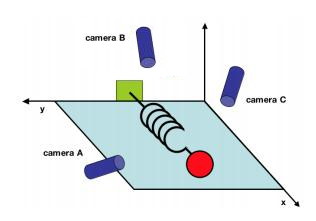
\includegraphics[scale=.75]{exampleSpring.jpg}
\caption{Toy example of an experiment on a spring system, taken from Shlens (2003).  \cite{shlens2003}. \label{fig.exampleSpring}}
\end{figure}

When we examine a dataset with a number (or dimensions) of predictors $p$, we may suspect that the data actually lie on a lower-dimensional manifold. For example, the three measurements of the previous setup were necessary to situate the ball on a spring but the data only had one true degree of freedom. Thus, rather than variable selection methods such as LASSO, we may want to consider more sophisticated techniques for learning the intrinsic dimensionality of the data, a field known as \emph{dimensionality reduction} or \emph{manifold learning}.

\section{Preliminaries in Linear Algebra and Statistics}

The above example and discussion  serve to motivate the introduction of \emph{Principal Component Analysis} (PCA).  In this section we give a brief overview of linear algebra and statistics, which were discussed in the first advanced section and are essential for the foundation of PCA.

\subsection{Linear Algebra}
For this section, let $X$ denote an arbitrary $n\times p$ matrix of real numbers, $X \in  {\Rset}^{n\times p}$. In these notes we assume that the reader is familiar with the basic matrix computations that are discussed in the first advanced section, such as matrix multiplication, transpose, row reduction, and
eigenvalue/eigenvector determination. 

\noindent
\paragraph*{\bf Proposition 1.1} \label{par:prop1.1} \textit{For any such matrix $X$, the matrices $X^T X$ and $X X^T$ are symmetric.}
\\
{\bf Proof:} To show symmetry of a matrix $A$ it suffices to show that $A^T = A$. Clearly, this holds in our case, since
\begin{align}
{(X^T X)}^T = X^T (X^T )^T = X^T X,
\end{align}
and similarly for $XX^T$. $\hfill \blacksquare$

The above proposition, while simple, is crucial due to an attractive property of real, symmetric matrices,  as it is given in the following theorem. Indeed, the following is often considered  as the fundamental theorem of linear algebra and  known as the \emph{spectral theorem}.

\noindent
\paragraph{\bf Theorem 1.2} \label{par:theor1.2} \textit{ If $A$ is a real, symmetric matrix, then there exists an orthonormal basis of eigenvectors of $A$.} 
\\ 
In order words, for any such matrix $A \in {\Rset}^{m\times m}$, we can find an eigenvector basis $ \{u_1 , . . . , u_m\}$ such that the basis is \emph{orthonormal}. That means that the basis vectors are orthogonal ($u_i \perp u_j$ so $u_i^T u_j  = \delta_{ij}$) and normalized to unity ($|| u_i ||_2 = 1$). Moreover, this basis consists of eigenvectors of $A$, so that $Au_i = \lambda_i u_i$ for the eigenvalue $\lambda_i \in \Rset$.
%
Alternatively, if we stack the eigenvectors $u_i$ as rows we obtain the orthogonal matrix   $U^T$, where  $U^T = U^{-1}$, and we can express the \emph{eigen-decomposition} of $A$ as 
\begin{align}
\label{eq:decomposition}
A = U\Lambda U^T,
\end{align}
where $\Lambda = \text{diag}(\lambda_i)$ is the diagonal matrix of eigenvalues.
%
The proof of the theorem is quite technical and we state the theorem here without proof. Moreover, there is a considerable amount of theory involving the set of eigenvalues of $A$, which is called its \emph{spectrum}. The spectrum of a matrix reveals much about its properties, and although we do not delve into it here, we encourage the reader to refer to the bibliography for further details.

We can, however, discuss one important property of the spectrum for the \emph{Gram matrices} $X^T X$ and $XX^T$; namely, that the eigenvalues are non-negative as the following preposition states.  

\noindent
\paragraph{\bf Proposition 1.3}\label{par:prop1.3} \textit{ The eigenvalues of $X^T X$ and $XX^T$ are non-negative reals.}
\\
{\bf Proof:} Suppose $\lambda$ is an eigenvalue of $X^T X$ with associated eigenvector $u$. Then,
\begin{align}
X^T X u &= \lambda u \nonumber \\ 
u^T X^T X u &= u^T \lambda u \nonumber \\
(X u)^T(X u) &= \lambda u^T  u \nonumber \\
||Xu||^2 &= \lambda ||u||^2 \nonumber \\
&\Rightarrow  \lambda >0
\end{align}
Since both $||X u||^2 $ and $||u||^2$ are non-negative, we conclude that $\lambda > 0$. Note that a zero eigenvalue implies that $X$ does not have full rank, since for $u \neq 0$, $X u = 0$ implies that the nullity (dimension of the null space) of $X$ is greater than 0. In these cases, the inverse of $X^T X$ does not exist. The result for $XX^T$ follows from a similar proof. $\hfill \blacksquare$

In fact, it turns out that the non-zero eigenvalues of these matrices are identical, as the following proposition shows.

\noindent
\paragraph{\bf Proposition 1.4}\label{par:prop1.4} \textit{The matrices $XX^T$ and $X^T X$ share the same nonzero eigenvalues.}
\\
{\bf Proof:}  Suppose that $\lambda$ is a non-zero eigenvalue of $X^TX$ with associated eigenvector $u$. Then
\begin{align}
X^T X u &= \lambda u\nonumber  \\
X X^T X u &=X \lambda u\nonumber  \\
X X^T (X u) &= \lambda (X u)\nonumber  \\
XX^T \tilde u &= \lambda \tilde u
\end{align}
Thus, $\lambda$ is  an eigenvalue of $X X^T$, with associated eigenvector $\tilde u = X u$ (rather than $u$).  $\hfill \blacksquare$

\paragraph{\bf Proposition 1.5}\label{par:prop1.5} \textit{The trace of the Gram matrix $X^TX$ is equal to the sum of its eigenvalues.}
\\
{\bf Proof:}  For the proof of \nameref{par:prop1.5}, we first prove the cyclic property of the Trace. Consider an $m\times n$ matrix $B$ and an $n\times m$ matrix $C$. Then, 
\begin{align}
\text{Tr }(BC) = \sum_i^m(BC)_{ii}=\sum_i^m\sum_j^n B_{ij} C_{ji}\nonumber \\
 \sum_i^m\sum_j^n  C_{ji} B_{ij} = \sum_j^n (CB)_{jj} = \text{Tr }(CB),
\end{align}
where we used the index notation for the trace and for the matrix multiplication. Invoking this property and using the eigen-decomposition of Eq. (\ref{eq:decomposition}), we prove \nameref{par:prop1.5}:
\begin{align}
\text{Tr }(X^T X) &= \text{Tr }(U\Lambda U^T) = \text{Tr }( U^TU\Lambda)=\text{Tr }( \Lambda)\nonumber \\
&\Rightarrow \text{Tr }(X^T X) = \sum_{i=1}^p \lambda_i.
\end{align}
Note that the above property holds for any Gram matrix. $\hfill \blacksquare$

\subsection{Statistics}

In this section, we return to considering $X\in \Rset^{n\times p}$ as the model matrix. From this point on, we assume that the predictors are all \emph{centered}, which means that for each column $X_j$ of $X$, we subtract the sample column mean
\begin{align}
\hat \mu_j = \frac{1}{n} \sumi x_{ij},
\end{align}
so that we are considering the centered model matrix:
\begin{align}
\tilde X =  \left( X_1-\hat \mu_1, ..., X_p-\hat \mu_p \right). 
\end{align}
Note that each column now has expectation zero, so that we can consider the \emph{sample covariance matrix}:
\begin{align}
S = \frac{1}{n-1} \tilde{X}^T \tilde{X}.
\end{align}
This is essentially a modified Gram matrix using the centered columns (or predictors) and scaling by  $n-1$. One way to understand the origin of its name is to consider each of the terms in the matrix. The diagonal matrix terms  all have the form:
\begin{align}
S_{jj} = \frac{1}{n-1}\sumi (x_{ij} - \hat \mu_j)^2 ,
\end{align}
whereas the off-diagonal terms have the form:
\begin{align}
S_{jk} = \frac{1}{n-1}\sumi (x_{ij} - \hat \mu_j)(x_{ik} - \hat \mu_k) .
\end{align}
Thus, it clear that the diagonal terms $S_{jj}$ yield the sample variances of each of the predictors, whereas the off-diagonal terms $S_{jk}$ yield the sample covariances.

\section{Principal Component Analysis}
\label{sec:pca}
With the above preliminaries, the actual methodology of PCA is now quite simple. The main idea is that in order to conduct dimensionality reduction and obtain the irreducible degrees of freedom inherent in the problem, we would like to remove as much redundancy in our predictors as possible. The way that PCA defines such redundancy is by using the correlation (or covariance) between the predictors. For instance, if predictors $x_j$ and $x_k$ are highly correlated, it is likely
that one holistic predictor may suffice instead.

Proceeding to the mathematics, we first use \nameref{par:prop1.1} to note that the sample covariance matrix $S$ is  symmetric and thus, we apply \nameref{par:theor1.2} to obtain an orthonormal basis of eigenvectors of $S$, such that the eigenvalues are ordered $\lambda_1 \ge  \lambda_2\ge...\lambda_p$ with corresponding eigenvectors $u_1 , u_2, ... , u_p$.
%
The vector $u_i$ is called the $i^\text{th}$ \emph{principal component} of $S$ and $\lambda_i$ is a measure of the "variance explained" by that principal component. This is because the trace of $S$,
\begin{align}
\tr{S} = \sum_{j=1}^p S_{jj} = \frac{1}{n-1} \sum_{j=1}^p \sumi (x_{ij} - \hat \mu_j)^2,
\end{align}
can be considered as the "total sample variance" of the predictors, as it sums up the sample variances of each of the $p$ predictor variables. But the trace of $S$ also equals the sum of its eigenvalues according to the \nameref{par:prop1.5}, hence, the quantity
\begin{align}
\frac{\lambda_i }{\sum_{j=1}^p\lambda_j}  = \frac{ \lambda_i }{ \tr{S}}
\end{align}
represents, in a heuristic sense, the fraction of the "total sample variance" accounted for  the eigenvector or principal component $u_i$.

In general, it will often be the case that the largest eigenvalues are orders of magnitude greater than the others, because the data may indeed have fewer degrees of freedom than the number of predictors may indicate. In practice, one keeps only the principal components with the largest eigenvalues, and discards the rest, thereby reducing the dimension of the problem, as shown in Fig. \ref{fig:examplePCA}. Thus, a smaller subset of the eigenvalues being significantly larger than the others indicates the possibility of dimensionality reduction. How many components to keep is left to the data analyst’s discretion, but it is generally clear when dimensionality reduction is possible.

\begin{figure}[ht!]
\centering
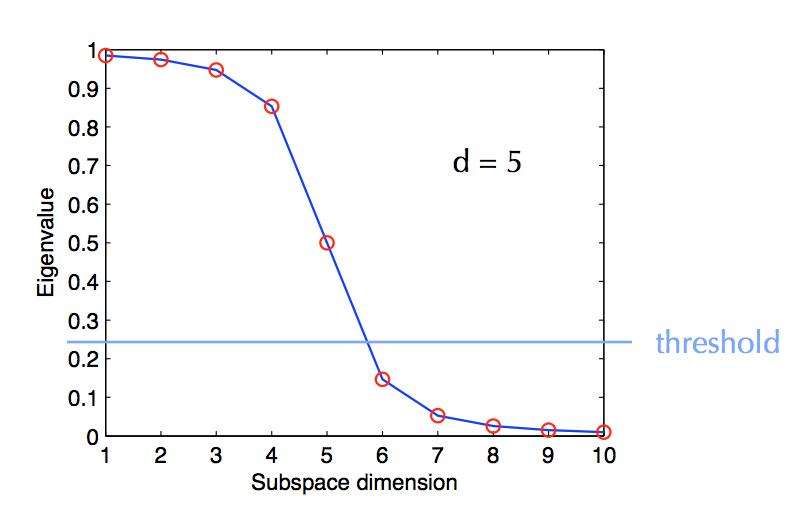
\includegraphics[scale=.5]{examplePCA.jpg}
\caption{An example of dimensionality reduction by PCA, thresholding the eigenvectors to keep based on examination of the eigenvalue magnitudes.} \label{fig:examplePCA}
\end{figure}

Intuitively, the principal components $u_i$ denote directions in $\Rset^p$ that are "natural" for the problem at hand, and are linear combinations of the original coordinates. For example, in the spring system example, we may  have $u_1 = (0.2, 0.9, 0.4)$ as the first principal component, which may have $\lambda_1/\sum_j \lambda_j \simeq 1$ revealing that there is just one degree of freedom as it represents the $x$-axis in Fig. \ref{fig.exampleSpring}. Consequently, the possibility of dimensionality reduction also indicates that there may be fewer but more interpretable variables, represented by the principal components, that are responsible for the variability of a response.

\section{Assumptions of Principal Component Analysis}

There are a number of assumptions that were both implicitly and explicitly made in order to motivate and justify the PCA method that is described in the previous section.
\begin{enumerate}[A.]
\item  \emph{Linear change of basis:} All of the operations that were used in section \ref{sec:pca}  are linear operations. Indeed, PCA consists essentially of a change of basis, from the Euclidean basis (in which we measure our predictors) to an orthonormal basis of eigenvectors of $X^T X$. Thus, PCA assumes that such a linear change of basis is sufficient for identifying degrees of freedom and conducting dimensionality reduction.

\item \emph{Mean/variance is sufficient:} In applying the PCA technique to our data, we are only using the means (for standardizing) and the covariance matrix that are associated with our predictors. Thus, the method assumes that such statistics are sufficient for describing the distributions of the predictor variables. This is, in fact, only the case if the predictors are drawn jointly from a multivariable Normal distribution, but may be approximately true in other situations. However, when the predictor distributions heavily violate this sufficiency assumption, one can still conduct PCA but the resulting components may not be as informative.

\item \emph{High variance indicates importance:} Another fundamental assumption that we made in describing PCA procedure is that the eigenvalues $\lambda_i$, which represent the variability in the data and are associated with the $i^\text{th}$ principal component, measure the importance of that component. This is intuitively reasonable, since components corresponding to low variability likely say little about the data, but this is not always true.

\item \emph{Principal components are orthogonal:} When were conducting PCA, we explicitly sought orthonormal eigenvectors as our principal components. The assumption that the "intrinsic dimensions" are orthogonal   may not be true. However, this allowed us to use techniques from linear algebra such as the spectral decomposition and thereby, simplify our calculations.
\end{enumerate}


Thus, while most of the assumptions appear plausible, they must be checked in practice before drawing any strong conclusions from PCA. Let us assess which assumptions are fundamental and which are technical. 
%
Assumption A is inherent in PCA, as a matrix-based method. Unfortunately, it is also one of the most limiting aspects of PCA. If the data are confined to a subspace, then linear methods will suffice. However, if the data are on some (nonlinear) manifold in the space, as put forth by the \emph{manifold hypothesis}, then linear methods are doomed to fail in general, and we must turn to nonlinear methods (see Section \ref{sec:NL}). 
%
Assumption B can be problematic, but unlike Assumption A, it can be more easily verified. For example, if any of the predictors appear to be heavily skewed, then the first two moments (mean and variance) are likely insufficient to describe the distribution, and thus PCA may not be very informative. In such a case, a transformation of certain problematic predictor variables (for example, by taking the logarithm) can be an adequate solution. Of course, one should ideally examine the joint distribution of the predictors, but this can be difficult in high-dimensional
situations. 
%
Finally, Assumptions C and D are not necessarily data-dependent, but rather method-dependent: that is, we make these assumptions as a way to understand the data, and they are not intrinsic to the data itself. Using metrics other than variability and allowing non-orthogonal components are not inherently nonsensical or antithetic to PCA; they will simply yield different methods and solutions to the problem of dimensionality reduction.



\section{Multidimensional Scaling and Other Linear Dimensionality Reduction Methods}

As noted above, PCA is a linear dimensionality reduction method that is based on a certain objective (maximizing variances and minimizing covariances), and substituting other metrics to be optimized yield  different methods \cite{saul2006}.  Rather than maximizing variances, one may want to instead find lower-dimensional representations of $X$ that preserve the \emph{pairwise distances} between the observations. This leads to the method of \emph{multidimensional scaling} (MDS).

As usual, suppose that we have $n$ observations $\{ x_1, . . . , x_n\} \subset \Rset^p $ , each of which are $p$-dimensional. Also, define a distance function between observations $d_{ij} = d(x_i, x_j )$, such that it is a \emph{metric}. Namely, it is symmetric $(d_{ij} = d_{ji})$, and has the property that $d_{ii} = 0$ and $d_{ij} > 0$ for $i \neq j$. Often, we will consider the Euclidean distance as our metric, so that $d(x_i , x_j ) = ||x_i - x_j||_2^2$ . One can verify that the Euclidean distance satisfies all properties necessary to be a metric. 

We can the construct the \emph{distance matrix} $D$, defined as 

\begin{equation}
\label{eq:X}
D  = 
 \begin{pmatrix}
  0 & d_{12} & \cdots & d_{1n} \\
  d_{21} & 0 & \cdots & d_{2n} \\
  \vdots  & \vdots  & \ddots & \vdots  \\
  d_{n1} & d_{n2} & \cdots & 0 \\
 \end{pmatrix},
 \end{equation}
where the diagonal terms are zero by definition of the metric. In addition, we can consider a lower-dimensional representation ${y_1, \cdots  , y_n } = {g(x_1 ), . . . , g(x_n )} \subset \Rset^d$ for $d < p$, and the associated distance matrix. We refer to the original distance matrix as $D^X$ and the distance matrix associated with the lower-dimensional representation as $D^Y$; note that both matrices are of dimension $n\times n$.

One criterion for ensuring that the lower-dimensional representation is faithful to the original data is to preserve the distances between the observations. Thus, in MDS, one seeks to find a representation such that
\begin{align*}
\stackunder{min}{g}\sum_{i,j=1}^n \left( d_{ij}^X - d_{ij}^Y\right)^2,
\end{align*}
where $g$ is the transformation that yields $y$. 

There are a number of ways one can use this framework for dimensionality reduction, but here we focus on the Euclidean case. In this situation, the following lemma connects the distance matrix to the Gram matrix $XX^T$:

\noindent
\paragraph*{\bf Lemma 5.1} \label{par:lemma5.1} \textit{The distance matrix $D$ for observations $\{x_1, . . . , x_n \}$ and Euclidean metric $d(x_i , x_j ) = || x_i - x_j ||^2_2 $ satisfies}
\begin{align}
XX^T = -\frac{1}{2}H D H,
\end{align}
\textit{where $H = I_n - n^{-1} \mathbf{11}^T$ where $\mathbf{1}$ is the vector of all ones.}

With the lemma \nameref{par:lemma5.1}, we can express the above minimization problem in terms of inner products as follows:
\begin{align}
\stackunder{min}{g}\sum_{i,j=1}^n \left(  x_i^Tx_j - y_i^Ty_j \right)^2,
\end{align}
and it can be shown that the solution to this problem is given by $Y =\Lambda^{ 1/2} V^T$ where $V$ is the matrix of eigenvectors corresponding to the largest $d$ eigenvalues of $XX^T$ , and $\Lambda$ is the diagonal matrix of those eigenvalues (and zero otherwise).
 
However, note from \nameref{par:prop1.4}  that, in fact, the largest $d$ eigenvalues of  $XX^T$ are exactly the largest $d$ eigenvalues of $X^T X$. Thus, despite approaching the problem from a completely different criterion, MDS actually yields the same dimensionality reduction as PCA. Thus, it is also a linear dimensionality reduction technique (if we use Euclidean distance as our metric) and suffers from the same drawbacks and assumptions as PCA.
 
 
\section{Nonlinear Dimensionality Reduction Techniques}
\label{sec:NL}

To surmount the linearity assumptions of PCA and MDS, there are, by now, a large number and variety of  \emph{nonlinear dimensionality reduction} techniques, which are also called \emph{manifold learning methods}. We focus on two salient examples of such methods, which are each based on one of the methods we have discussed.

\subsection{Kernel PCA}
One obvious extension to PCA that allows for nonlinear dimensionality reduction is to first apply a nonlinear map $\Phi$, known as a \emph{feature map} to the data, yielding a nonlinear representation $\Phi(X)$, then applying PCA to this transformed data.  Once we transform the data, we must find the Gram matrix in this transformed space, which we define to be the \emph{kernel}:
\begin{align}
K = \Phi(X)^T \Phi(X).
\end{align}
Once we have achieved this, we can conduct PCA on this Gram matrix, just taking care to ensure that the columns have mean zero. This yields the kernel PCA method for nonlinear dimensionality reduction.

Note that we cannot simply standardize each column as before, since that does not conform to the transformation above. Instead, we must modify the feature map itself as:
\begin{align}
\tilde{\Phi}(X) = \Phi(X) - \Ep{x}{\Phi(X)},
\end{align}
and then compute the modified kernel $\tilde{K} = \tilde{\Phi}(X)^T \tilde{\Phi}(X)$.


\subsection{Isomap}
Similarly to the case of kernel PCA, one can extend MDS to the nonlinear setting by using a non-Euclidean distance metric. One widely-used alternative yields a technique called \emph{Isomap}. The exact same MDS objective is minimized as before (minimizing the difference in pairwise distances between the original points and the transformed representation). However, we employ a different, particular distance metric $d(x_i , x_j)$.

To construct this metric, one first constructs the $k$-nearest neighbors (KNN) graph of the data. This entails employing the KNN method on the data, and constructing a graph in which the data points are the nodes, and an undirected edge $\{i, j\}$ indicates that $(x_i , x_j)$ are one of each other’s $k$-nearest neighbors. Then, one can use a shortest-paths algorithm (such as Djikstra’s algorithm) to compute the shortest geodesic distance between pairs of observations. That is, $d_{ij} = d(x_i , x_j )$ indicates the length of the shortest path between $x_i$ and $x_j$ in this nearest neighbors graph.

Finally, one can use a standard optimization algorithm or an eigen-decomposition of the distance matrix $D^X$ to find the representations $Y$. This step is identical to that of MDS, and it is noted that one can use the number of "large" eigenvalues of $D^X$ to determine the dimensionality of the representation.


\begin{thebibliography}{99}
\bibitem{bishopBook} C. Bishop, \textit{Pattern Recognition and Machine Learning}, 8th ed. Springer (2008).
\bibitem{shlens2003} J. Shlens,  \textit{A Tutorial on Principal Component Analysis}, (2003).
\bibitem{jauregui2012} J. Jauregui, \textit{Principal component analysis with linear algebra}, (2012).
\bibitem{saul2006} L. K. Saul, et al. \textit{Spectral Methods for Dimensionality Reduction}, Semisupervised Learning, 293-308 (2006).
\end{thebibliography}
\end{document}
